\documentclass[11pt,UTF8]{report}

\usepackage{ctex}

\usepackage{listings}
\usepackage{xcolor}

\usepackage{graphicx}

\usepackage[colorlinks, linkcolor=red, anchorcolor=blue, citecolor=green]{hyperref}

\lstset{
    basicstyle=\tt,
    %行号
%    numbers=left,
%    rulesepcolor=\color{red!20!green!20!blue!20},
%    escapeinside=``,
%    xleftmargin=2em,xrightmargin=2em, aboveskip=1em,
    %背景框
%    framexleftmargin=1.5mm,
%    frame=shadowbox,
    %背景色
%    backgroundcolor=\color[RGB]{245,245,244},
    %样式
    keywordstyle=\color{blue}\bfseries,
    identifierstyle=\bf,
    numberstyle=\color[RGB]{0,192,192},
    commentstyle=\it\color[RGB]{96,96,96},
    stringstyle=\rmfamily\slshape\color[RGB]{128,0,0},
    %显示空格
    showstringspaces=false
}

\renewcommand\thesection{\arabic{section}}

\title{数据库系统概论大作业报告}
\author{杜政晓 2016011014\\
吴一凡 2016011269}
\begin{document}
\maketitle

\section{系统概述}
Github地址\url{https://github.com/duzx16/MyDB}
\subsection{必做功能}
\begin{itemize}
	\item 基于页式文件的记录管理
	\item \emph{基于页式文件}的B+树索引
	\item 数据库,关系表,索引的创建和删除
	\item 关系表中数据的增删查改
\end{itemize}

\subsection{选做功能}
\begin{itemize}
	\item 属性域约束(check)和外键约束
	\item 支持Date数据类型(Date)
	\item 三个或以上表的连接,并支持使用索引加速
	\item 聚集查询函数AVG, SUM, MIN, MAX和分组查询GROUP BY
	\item 模糊查询,基于LIKE和"\%","\_"的通配查询
	\item 更灵活的查询语句,支持使用任意的逻辑表达式作为查询条件
\end{itemize}

\section{系统架构设计}
\begin{figure}[!ht]
	\centering
	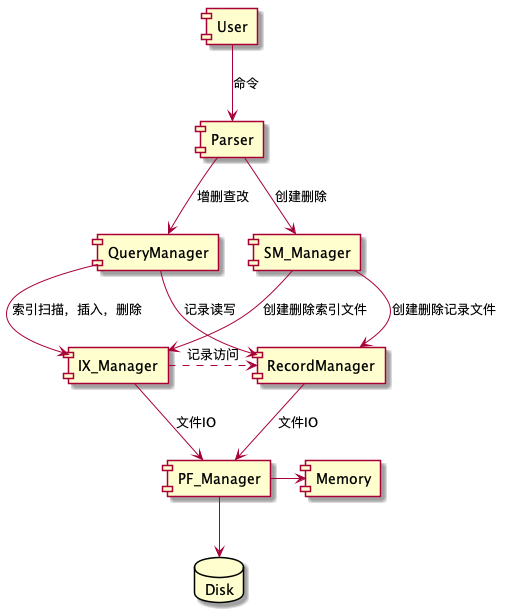
\includegraphics[width=0.9\textwidth]{structure}
	\caption{系统架构设计图}
	\label{fig:structure}
\end{figure}

整个数据库系统的架构设计和CS346以及《数据库大作业详细说明》中一样。最底层是一个页式文件管理系统,负责以页为单位进行磁盘文件的读取,写入和缓存。建立在其上的是记录管理系统(负责管理数据表中的记录的创建,插入,删除,修改)和索引管理系统(负责管理数据表中属性索引的创建,插入,删除)。然后用户的指令由Parser解读,其中对数据表和索引的创建、删除的指令由系统管理模块处理,对数据的增删查改由查询处理模块处理。具体的架构图见图\ref{fig:structure}.

\section{各模块详细设计}
\subsection{记录管理模块}
\subsubsection{文件结构设计}
每个文件只存储同一类长度相等的记录。文件由页(Page)组成,,页由大小等于记录长度的槽(Slot)组成。
每个文件的第一页作为文件头,保存了文件的一些元信息,比如记录长度、文件中的页数目、文件中的记录数目等。
文件中每一页的开头保存了该页的一些基本信息。比如该页的槽哪些是空的哪些是非空的。这里使用了Bitmap来表示槽的空与非空。此外,为了能够在插入记录的时候能够快速找到有空槽的页,使用了一个链表来存储有空槽的页。首页中保存了链表中的第一项的页码。每一页的开头4个字节指向的是链表中下一项的页码。比起在首页中用Bitmap来表示页是否非空,这种方式能够存储的页数是没有限制的。

\subsubsection{模块具体实现}

因为在使用提供的页式文件管理系统的时候出现了奇怪的bug(具体表现是缓存的hash表有时候会突然“丢掉”某个已经打开的页,导致该页对应的页数变成了一个随机数)。而且该文件系统的功能不全(比如没有将某个页固定在缓存中不要换出的功能,在关闭文件的时候也不会写回它的所有页),所以我换用了CS346中提供的页式文件管理系统。
RecordManager的创建、删除文件都使用文件管理系统的接口。打开文件除了调用接口外,还会将文件的首页中的信息复制出来,并设置modified为false。如果后续操作中改变了首页信息则将modified设置为true。当关闭文件的时候,如果发现modified为true,则将复制出来的信息写回文件的首页。
RM\_FileHandle负责对文件中的记录进行管理。插入记录时,从首页中找到有空槽的页,然后进行插入。如果发现插入之后该页已经满了,则将首页上有空槽的页码换为链表中的下一项。在删除记录的时候,只需要将Bitmap的对应位设置为空,然后将该页的页码插入到链表的开头。
对文件的扫描由RM\_FileScan进行,其方法就是依次遍历每一页,每一页中遍历Bitmap中的每一个非空位对应的槽。

\subsection{索引管理模块}

在CS346的模块设计中,索引管理模块维护的是属性值的指针以及该属性值对应的记录在记录文件中的RID的二元组。这样做主要意在实现记录管理模块及索引管理模块的分离。但如果按照这种设计的话,要将所有插入进来的属性值在索引文件中再存一遍。这样做不仅效率较低,也不方便实现,还会浪费空间。因此决定将索引管理模块的接口改为仅维护属性值对应的记录在记录文件中的RID,也就是说只要提供RID就可以进行插入和删除。但为了知道属性值的类型以及从记录文件中获取属性值的指针,在打开索引时还需要提供一个已经打开的RM\_FileHandle以及该属性值开头在所有属性值中的偏移量。

于是索引管理模块的功能为,在一个已经打开的记录文件以及属性的偏移量已知的情况下,可以基于RID来插入/删除索引,也可以给定一个条件(目前支持$<,\leq,>,\geq,=,\not=,\text{NO\_OP}$这几种运算符)以及比较值来对所有符合条件的属性值对应的RID进行遍历。
\subsubsection{文件结构设计}

将整个索引仅存在一个索引文件中,其中第一页存的是描述属性类型、属性字节数、B+树根节点的页码的索引信息。剩下的所有页要么存的是包含内部节点及叶子节点的B+树节点,要么存的是属性值同为某一个值的所有RID。由于在实现中将这些RID都只存在一页中,所以属性值相同的RID数目不能过多。
\subsubsection{模块具体实现}

索引管理模块使用B+树对索引进行维护。对于B+树的讨论在这里就不再赘述了。值得注意的是为了实现简便,在对索引进行删除时并未进行下溢的节点合并处理。虽然在理论上可能有些小问题,但经过测试,这样的实现也是可以接受的。

在进行遍历时,首先找到B+树中最小的$\geq$比较值的属性值对应的RID的位置,随后根据运算符向左或者向右一步一步找到所有符合要求的RID。注意这里将所有符合要求的RID都预先存了下来,因此在遍历过程中插入或删除索引并不会影响索引的遍历。但由于索引是基于记录的,若要同时修改记录与索引,应先修改索引,再修改记录。

\subsubsection{测试程序}

为了验证该模块的正确性,实现了一个ix\_test.cc来进行测试,如果不对的话就会assert退出。
\subsection{系统管理模块}

系统管理模块作为页式文件系统、记录管理模块、索引管理模块的客户端,负责调用上述三个模块处理SQL解析器解析到的部分命令。这些命令有:

\begin{itemize}
	\item 创建/删除数据库
	\item 打开/关闭数据库
	\item 创建/删除表
	\item 创建/删除索引
	\item 打印(所有)表信息
\end{itemize}
\subsubsection{文件结构设计}

每个数据库都对应一个与数据库名字相同的数据库主程序目录下的子文件夹,该数据库的所有信息都存在这个子文件夹下,其中包含一个TableList文件存数据库的所有表的名字,且对于每个表存表的信息文件(包括表的所有属性及约束,每个属性是否被索引)、表的记录文件、表的索引文件(每个属性的索引一个文件)。
\subsubsection{模块具体实现}

创建/删除数据库实际上就是创建/删除文件夹,打开/关闭数据库实际上就是进入/退出子文件夹。创建表时我们需要将表的名字插入TableList文件,同时新建并修改表的信息文件,将表的属性与约束写入表的信息文件;删除表时则删除所有跟表有关的文件,并在TableList中删除表名。创建索引时调用索引管理模块的创建索引功能,并且打开记录文件遍历所有的RID并依次调用索引管理模块的插入索引功能进行插入,并将该属性修改为被索引;删除索引则正好相反。打印表信息只需打开表的信息文件并输出即可。
\subsection{SQL解析器}
Parser使用flex + bison (Yacc的升级版)实现, 其语法大致与本课程给出的Parser语法文件相同。但是进行了以下拓展:
\begin{itemize}
	\item 在create table的时候, 除了主键和外键, 还可以指定属性域约束check in, 此外主键约束可以用多个域连接作为主键。
	\item select语句支持group by关键词, 以及SUM, AVG, MIN, MAX等函数。
	\item insert语句支持指定插入哪些列(未指定的列自动视为null)。
	\item where子句中支持任意的涉及四则运算的表达式, 只要最终结果是布尔类型(原语法只支持用and连接的column comp value的比较)。 增加like比较运算。 update的set子句的右半部分也可以是任意类型兼容的四则运算表达式。
\end{itemize}

Parser在完成解析之后会根据语句生成对应的类, 然后调用相应的模块进行执行。

\subsection{查询处理模块}
查询解析模块是整个数据库中最重要也是最复杂的一个部分, 用户在使用的数据库的时候主要都是在和查询解析模块打交道。查询解析模块主要有三个类:Expr,Table和QueryManage。

\subsubsection{Expr}
因为我们支持的表达式比较复杂,所以我们单独设计了Expr类,表示由代数运算(+-*/), 比较(<>=), 逻辑运算(AND OR)组成,以常量或者是表的列为叶子的抽象语法树. 其类型包括代数表达式, 比较表达式, 逻辑表达式, 常量, 关系表属性. 支持以下功能:
\begin{itemize}
	\item 绑定到关系表的某项属性, 给定数据之后自底向上进行计算。
	\item 逻辑运算支持短路操作, 对于某些where子句可以提前计算出结果, 减少遍历的时间
	\item 进行必要的类型兼容检查, 并在必要时将整型数据向浮点类型提升
	\item 通过重载运算符在两个Expr之间进行简单的运算和比较(主要是方便聚合函数)
	\item 按照一定的规则转化为格式化的字符串。其中对于INT类型的属性,可以指定长度。
	\item 提供后序遍历的接口来扩展
	\item \textbf{支持字符串的like匹配:} 为扩展功能中的like关键字提供匹配。实现方法是将SQL语句中的"\_"和"\%"用正则表达式中的"\."和"\.\*"来替换,然后调用C++11中的regex模块进行正则表达式的匹配。
	\item \textbf{支持字符串向Date的转化:} 将一个xxxx-xx-xx类型的字符串转化为一个4字节整数,便于在数据库中存储。并进行日期合法性的检查。
\end{itemize}

\subsubsection{Table}
Table模块在《数据库大作业详细说明》中给出的数据库架构是不存在的. 但是考虑到其他三个模块中都没有关系表这个概念, 而查询解析模块的四大功能中又要用到很多共同的功能, 所以在程序中加入了数据库中关系表对应的类Table. 通过调用其他三个模块来提供以下功能:
\begin{itemize}
	\item 管理一个关系表相关的记录文件和索引文件handler, 避免重复打开和关闭。同时在析构的时候自动释放申请的资源。
	\item 查询关系表的属性域的信息, 如长度, 偏移量, 约束等。
	\item \textbf{检查记录是否符合关系表上的约束:} 其中,主键约束和外键约束通过对应属性的索引来检查当前值是否已经存在(因为主键一定有索引,外键一定是其他表的主键,所以不用担心索引未创建)。属性域约束只需要检查当前值是否等于给定的常量列表中的某一个值。
	\item 将insert的常量转化为连续的数据, 并进行约束检查。如果约束检查通过,则作为记录插入,并将属性值插入到已经创建的索引中。
	\item 根据set子句更新给定的记录,并进行约束检查。如果约束检查通过,则更新记录文件,并更新对应属性的索引(通过先删除再插入的方式)。
\end{itemize}

\subsubsection{QueryManager}
\subsubsection{表的遍历}
查询处理模块首先提供了一个基础的方法iterateTables, 用于提供对一个关系表或多个关系表的连接进行有筛选的遍历的接口, 通过传入一个回调函数来对记录进行操作。

这个函数有两个版本, 一个是对于最常用的单表遍历(update, delete都只会调用这个函数). 对于单表遍历来说, 利用索引的方式是找到那些where子句中必须满足的比较条件, 并且左边是某个有索引的属性域, 右边是一个常量, 然后就可以用索引模块提供的接口来直接查找符合这一条件的记录。如果找不到这样的比较条件,则直接全部遍历。将遍历到的记录的数据用Expr的calculate功能算出条件表达式的值,完成筛选。

另一个是对于任意多的表连接进行遍历(select可能会调用这个函数). 利用索引的方式同样是找到where子句中必须满足的比较条件, 左边是某个有索引的属性域, 右边的表达式不含有跟左边同一个关系表的属性, 并且出现的关系表尽可能少(常量是最好的情况, 不出现任何关系表). 然后在安排局部的遍历顺序的时候, 把出现在右边的关系表都安排在外层, 然后到了遍历左边的关系表的时候就可以利用其索引. 当然这种方法其实是一种贪心的方法, 一旦表的数量较多, 并不能保证效率是最高的. 不过考虑到我们只是一个教学用的数据库, 不会进行太多表的连接, 所以也可以满足要求了.

\subsubsection{插入,修改与删除}
在四大功能中, insert不需要遍历, 直接调用Table的接口向记录文件和索引文件中插入就可以了。update和delete都只需要单表遍历, update和delete都首先将遍历到的记录的RID储存起来(避免在遍历表的过程中修改索引的结构),遍历结束后再统一调用Table的接口进行修改或删除。

\subsubsection{聚集函数}
为了便于聚集函数的查询,我们实现了Aggregation类来实现聚集函数的功能。其提供的接口accumulate(const std::string \&group, const Expr \&value)表示遇到一个新的值。对于非group查询来说,直接统计对应的统计量(AVG, SUM, MIN, MAX),对于group查询来说,先将group attribute统一转化成字符串,然后利用C++的std::map来实现从group attribute到对应统计量的映射。

\section{主要接口说明}
\subsection{记录管理模块}
记录管理模块的核心是类RecordManager,用于实现记录管理中文件级别的操作,其接口包括:
\begin{lstlisting}[language=C++]
// Create a file with filename and record size
int createFile (std::string filename, unsigned record_size);
// Delete a file with filename
int destroyFile(std::string filename);
// Open a file with filename in file_handle
int openFile(std::string filename, RM_FileHandle &file_handle);
// Close the file opened in file_handle
int closeFile(RM_FileHandle &file_handle);
​\end{lstlisting}

通过RecordManager打开的文件会返回一个RM\_FileHandle,用于实现对于单个文件中记录的操作
\begin{lstlisting}[language=C++]
// Get a record by rid
int getRec(const RID &rid, RM_Record & record) const;
// Insert a new record and return the rid
RID insertRec(const char *pData);
// Delete a record by rid
int deleteRec(const RID &rid);
// Update a record
int updateRec(const RM_Record &rec);
\end{lstlisting}

此外还有一个类RM\_FileScan用来进行对文件中记录的查询
\begin{lstlisting}[language=C++]
// Initialize file scan
int openScan(const RM_FileHandle &fileHandle,
             AttrType attrType,
             int attrLength,
             int attrOffset,
             CompOp compOp,
             void *value
);
// Get next matching record
int getNextRec(RM_Record &rec);
// Terminate file scan
int closeScan();
\end{lstlisting}

注意在记录管理模块中我们只实现了对记录中单个属性值进行限制的查询。
\subsection{索引管理模块}
IX\_Manager类可以创建/删除索引,并可以在给定一个打开的RM\_FileHandle以及属性偏移量的情况下打开IX\_IndexHandle类型的索引,也可以关闭索引。
\begin{lstlisting}[language=C++]
// Create new index
RC CreateIndex (const char *fileName,          
                int indexNo,
                AttrType attrType,
                int attrLength);
// Destroy index
RC DestroyIndex (const char *fileName,          
                 int indexNo);
 // Open index
RC OpenIndex    (const char *fileName,         
                 int indexNo,
                 IX_IndexHandle &indexHandle,
                 RM_FileHandle &rmFileHandle,
                 int _attrOffset);
// Close index
RC CloseIndex   (IX_IndexHandle &indexHandle);  
\end{lstlisting}
IX\_IndexScan类可以在给定一个打开的IX\_IndexHandle以及比较运算符与比较值的情况下打开,并通过GetNext对所有符合条件的RID进行遍历。                           
\begin{lstlisting}[language=C++]
// Initialize index scan
RC OpenScan(IX_IndexHandle &indexHandle, 
             CompOp compOp,
             const void *value,
             ClientHint  pinHint = ClientHint::NO_HINT);
// Get next matching entry
RC GetNextEntry(RID &rid); 
// Terminate index scan                       
RC CloseScan();     	
\end{lstlisting}
\subsection{系统管理模块}
系统管理模块SM\_Manager暴露给调用者parser的接口有:
\begin{lstlisting}[language=C++]
RC CreateDb(const char *dbName);             
RC DropDb(const char *dbName);             
RC OpenDb(const char *dbName);            
RC CloseDb();                                  
RC CreateTable(const char *tableName,
               ColumnDecsList *columns,
               TableConstraintList *tableConstraints);
RC GetTableInfo(const char *tableName,
                ColumnDecsList &columns,
                TableConstraintList &tableConstraints);				
RC DropTable(const char *relName);               
RC CreateIndex(const char *relName, const char *attrName);
RC DropIndex(const char *relName, const char *attrName);
// Help for database
RC Help();        
// Help for relation                          
RC Help(const char *relName);               	
\end{lstlisting}
\subsection{查询处理模块}
查询处理模块对外的类只有QueryManager,其public方法分别对应于数据库的增删查改
\begin{lstlisting}[language=C++]
// select attributes on relations 
// with (possibly empty) where condition and group attributes
int exeSelect(AttributeList *attributes, IdentList *relations,
 Expr *whereClause, const std::string &groupAttrName);
// insert into relation table(可以用columnList指定要插入的列)
int exeInsert(std::string relation, IdentList *columnList, 
ConstValueLists *insertValueTree);
// update relation table as setClauses with where condition
int exeUpdate(std::string relation, SetClauseList *setClauses,
 Expr *whereClause);
// delete the data in relation table with where condition
int exeDelete(std::string relation, Expr *whereClause);

\end{lstlisting}


\section{实验结果}
程序的编译运行方法见readme.md。基于本课程给出的dataset\_small,我们编写了4组测试语句。位于test文件夹下。从运行结果中可以看出我们的数据库完成了Section 1中描述的功能,且能在较短的时间内完成多表遍历等复杂的操作。

\section{小组分工}
\begin{itemize}
	\item 杜政晓:记录管理模块,查询处理模块,SQL parser
	\item 吴一凡:索引管理模块,系统管理模块
\end{itemize}

\section{参考文献}
\begin{itemize}
	\item 《数据库大作业详细说明》
	\item CS346 RedBase Project \url{https://web.stanford.edu/class/cs346/2015/redbase.html}
	\item SimpleDB by Harry Chen \url{https://github.com/Harry-Chen/SimpleDB}
	\item database by 马也 \url{https://git.net9.org/maye9999/database}
	\item STX B+ Tree Template \url{https://panthema.net/2007/stx-btree}
\end{itemize}
\end{document}
